\documentclass[12pt,a4paper]{report}
\usepackage{color}
\usepackage[utf8]{inputenc}
\usepackage[dvipsnames]{xcolor}
\usepackage[dutch]{babel}
\usepackage[margin=1in]{geometry}
\usepackage[pdftex]{graphicx}
\usepackage{titlesec}
\usepackage{titletoc}
\usepackage{imakeidx}
\usepackage{listings}
\usepackage{hyperref}
\definecolor{darkblue}{rgb}{0,0,0.5} 
\hypersetup{
	linktoc=all,
	colorlinks=true,    % false: boxed links; true: colored links
	linkcolor=darkblue, % color of internal links (change box color with linkbordercolor)
	citecolor=darkblue, % color of links to bibliography
	filecolor=magenta,  % color of file links
	urlcolor=blue       % color of external links
}
\usepackage{syntax}
\usepackage{amsmath}
\usepackage{breakurl}

\makeindex

\setcounter{tocdepth}{2}

\titleformat{\chapter}[display]{\normalfont\huge\bfseries}{\chaptertitlename\ \thechapter}{18pt}{\huge}
\titlespacing*{\chapter}{0pt}{20pt}{20pt}

\begin{document}
\lstset{ %
  breakatwhitespace=true,
  breaklines=true,
  commentstyle=\color{gray},
  frame=single,
  keepspaces=true,
  language=Haskell,
  numbers=left,
  numbersep=5pt,
  numberstyle=\color{gray},
  showspaces=false
}

\pagenumbering{arabic}
\topskip0pt
\vspace*{\fill}
\begin{center}
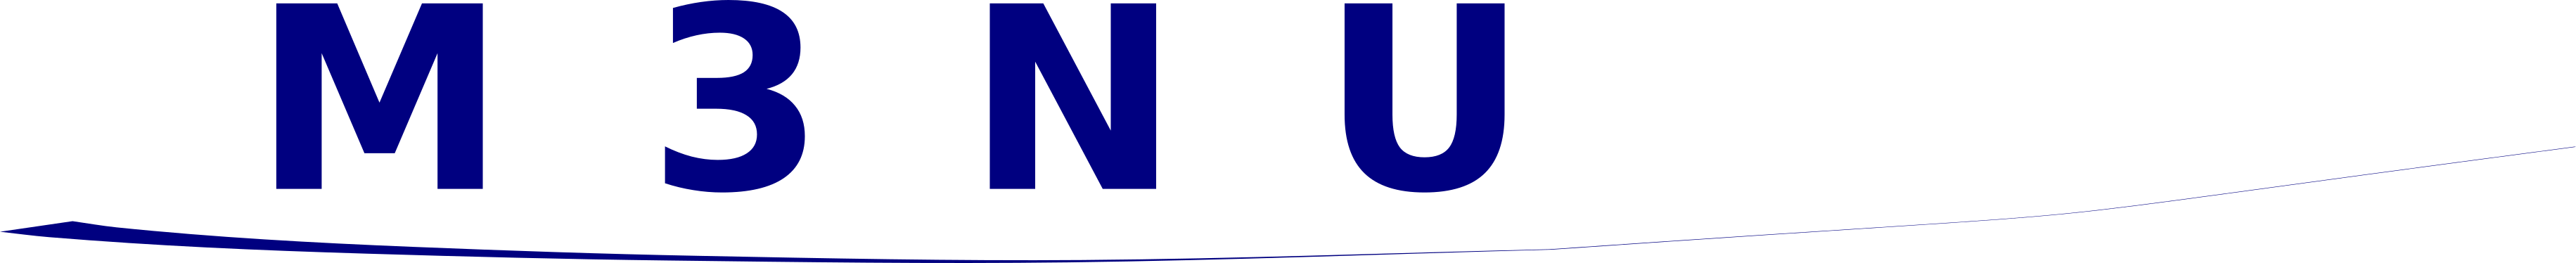
\includegraphics[width=100mm]{verslag/logo.png}
\vspace*{1.5in}\\
  {\Huge Functioneel Programmeren}\\
  {\Large Pieter De Clercq}
\end{center}
\vspace*{\fill}
\begin{center}
% Include university logo at exactly the right size

\includegraphics[width=53mm]{verslag/logo-ugent.pdf}
% Include faculty logo at exactly the right size

\includegraphics[width=74mm]{verslag/logo-we.pdf}
\end{center}
\tableofcontents
\newpage
\chapter{Inleiding}
De syntax van deze taal vindt zijn oorsprong in een schematisch idee op papier. Aangezien mijn schema's doorgaans uitpuilen van de pijltjes, zijn deze blijven staan in de uiteindelijke implementatie van de taal. De naam M3NU is afkomstig van het woord Menu en alle identifiers en keywords zijn gebaseerd op culinaire termen. Oorspronkelijk waren de namen van MBot statements simpelweg ``leds'' en ``drive'', maar Ruben Maes besloot mij van inspiratie te voorzien voor nieuwe namen, waarvoor dank. Inspiratie voor de werking van de taal heb ik geput uit de bestaande talen waarin ik het liefst programmeer, namelijk C, PHP en Python. Een resultaat hiervan is dat booleans geïmplementeerd zijn als getallen 1 en 0, respectievelijk true en false. Elke aritmetische expressie die niet naar 0 evalueert, wordt booleaans true, equivalent aan de implementatie in Python. Als bestandsextensie werd voor .course gekozen, het Engelse woord voor een ``gang'' in een menu.
\chapter{Syntaxis}
arrow $::= ->$\\
end $::= $`;'\\
\section{Getallen}
digit $::= 0|1|2|...|9$\\
commasep $::= .$\\
neg $::= -$\\
number $::= \{digit\}_{1+}$ $|$ $\{digit\}_{1+}\{commasep\}_{1}\{digit\}_{1+}$\\
sgnnumber $::= \{number\}_{1}$ $|$ $\{neg\}_{1}\{number\}_{1}$\\

\section{Expressies}
lowercase $::= a|b|c|...|z$\\
uppercase $::= A|B|C|...|Z$\\
letter $::= \{lowercase\}_{1} | \{uppercase\}_{1}$\\
variable $::= \{letter|digit\}_{1+}$\\
bool $::= tasty$ $|$ $disguisting$\\
opa $::= +$ $|$ $-$ $|$ $*$ $|$ $/$\\
opb $::= and$ $|$ $or$\\
opr $::= >|>=|==|<=|<$\\
operator $::= \{opa\}_{1} | \{opb\}_{1} | \{opr\}_{1}$\\
exppart $::= \{sgnnumber\}_{1} | \{variable\}_{1} | \{bool\}_{1} | \{mbotSensor\}_{1} | \{(exppart)\}_{1}$\\
unexp $::= $`|' $\{exp\}_{1}$ `|' $| !\{exp\}_{1} | (\{unexp\}_{1})$\\
binexp $::= (\{exp\}_{1} \{operator\}_{1} \{exp\}_{1})$\\
exp $::= \{exppart\}_{1} | \{binexp\}_{1} | \{(exp)\}_{1}$\\

\section{MBot}
knowncol $::= red$ $|$ $green$ $|$ $blue$ $|$ $cyan$ $|$ $magenta$ $|$ $yellow$ $|$ $white$\\
rgbcol $::= \{exp\}_{1}, \{exp\}_{1}, \{exp\}_{1}$\\
color $::= \{knowncol\}_{1} | \{rgbcol\}_{1}$\\
direction $::= forward$ $|$ $left$ $|$ $right$ $|$ $backward$ $|$ $backwardleft$ $|$ $backwardright$ \\
\indent\indent\indent$|$ $brake$\\
leds $::= left$ $|$ $right$\\
mbotSensor $::= linesensor | ultrason$\\
mbotLed $::= colalight \{leds\}_{1} \{arrow\} \{color\}_{1} \{end\}_{1+}$\\
\indent\indent\indent$| colazero \{leds\}_{1} \{end\}_{1+}$\\
mbotDrive $::= drivethrough \{direction\}_{1} \{end\}_{1+}$\\

\section{Statements}
cookStmt $::= cook \{exp\}_{1} \{end\}_{1+}$\\
eatingStmt $::= eating \{exp\}_{1} \{arrow\}_{1} \{stmt\}_{0+} enough \{end\}_{1+}$\\
hungryStuffed $::= hungry \{exp\}_{1} \{arrow\}_{1} \{stmt\}_{0+}$\\
\indent\indent\indent\indent $stuffed \{arrow\}_{1} \{stmt\}_{0+} satisfied \{end\}_{1+}$\\
hungryNotStuffed $::= hungry \{exp\}_{1} \{arrow\}_{1} \{stmt\}_{0+} satisfied \{end\}_{1+}$\\
hungryStmt $::= \{hungryStuffed\}_{1} | \{hungryNotStuffed\}_{1}$\\
orderStmt $::= order \{variable\}_{1} \{arrow\}_{1} \{exp\}_{1} \{end\}_{1+}$\\
pukeStmt $::= puke \{exp\}_{1} \{end\}_{1+}$\\
reviewStmt $::= review \{any_character\}_{0+} \{end\}_{1+}$\\
stmt $::= \{cookStmt\}_{1} | \{eatingStmt\}_{1} | \{hungryStmt\}_{1} | \{orderStmt\}_{1} | \{pukeStmt\}_{1}$\\
\indent\indent$| \{reviewStmt\}_{1} | \{stmt\}_{1+}$\\

\chapter{Semantische constructies}
\section{Cook}
Dit statement biedt de mogelijkheid om de uitvoering van het programma te pauzeren voor een gegeven tijdsspanne, uitgedrukt in seconden. De naamgeving voor deze methode komt van de eenvoudige logica, dat er iemand niet kan eten terwijl die aan het koken is, dus de thread waarop het programma draait ook niet.

\section{Eating}
While-lussen kunnen gebruikt worden door middel van ``Eating''-statements. De werking is niet anders dan bij andere programmeertalen; een blok code wordt uitgevoerd zolang een conditie naar ``true'', tasty, evalueert.

\section{Hungry}
De traditionele ``if-else''-controlestructuur werd geïmplementeerd door het ``hungry-stuffed''-statement. Als de expressie naar ``tasty'' evalueert wordt de ``hungry''-tak uitgevoerd, anders de ``stuffed''-tak. Een noemenswaardig verschil met Haskell is dat de ``else/stuffed''-tak van het statement hier optioneel is, terwijl dit in Haskell verplicht is.

\section{Order}
Assignment gebeurt met het ``Order''-statement. Variabelen worden gestockeerd in de environment en kunnen later in expressies weer gebruikt worden. Scoping van variabelen is niet mogelijk, alles zit in de global scope. Mocht ik functies willen implementeren, zou ik er hoogstwaarschijnlijk voor opteren dit zo te houden aangezien de code een heel stuk gecompliceerder zou worden met ondersteuning voor scope.

\section{Puke}
Met het ``Puke''-statement kan uitvoer naar de console, met andere woorden naar ``standaard-uit'' weggeschreven worden. Zowel booleaanse als aritmetische expressies, alsook sensorwaarden kunnen worden getoond. De naamgeving van dit statement is vrij voordehandliggend, maar toch is er nog een diepere betekenis. Het woord ``Puke'' heeft namelijk een eerder negatieve connotatie; dit in overeenstemming met het feit dat I/O over het algemeen traag en bijgevolg negatief is.

\section{Review}
Commentaar is mogelijk via het ``Review'' statement. Ondersteuning voor commentaar op willekeurige plaatsen in de code is niet ingebouwd. De ondersteunde vormen van commentaar zijn lijncommentaar en commentaar over meerdere lijnen. Commentaar over meerdere lijnen is een logisch resultaat van \textsc{5.2.} en vereiste geen verdere aanpassing aan de code.

\section{Drivethrough (MBot)}
Met dit commando worden de motoren van de MBot aangestuurd. De motoren individueel aansturen is niet mogelijk, wel kan er eenvoudig gestuurd worden door een richting mee te geven aan dit statement. Ondersteunde richtingen zijn ``forward'', ``left'', ``right'', ``backward'', ``backwardleft'', ``backwardright''. De motoren stoppen, remmen, is ook mogelijk met de richting ``brake''.

\section{Leds (MBot)}
Om de LED's van de MBot te controleren werden twee statements ingevoerd. Met het ``colalight'' statement kunnen de LED's afzonderlijk ingeschakeld worden en een kleur krijgen, met het ``colazero'' statement kunnen de LED's worden uitgeschakeld. Kleuren kunnen uitgedrukt in RGB-waarden, maar er zijn ook enkele basiskleuren ingebouwd. Deze zijn ``red'', ``green'', ``blue'', ``cyan'', ``magenta'', ``yellow'', ``white''.

\section{Sensoren (MBot)}
De waarden lijnsensor en ultrasonische sensor kunnen worden opgevraagd met de expressies ``linesensor'' en ``ultrason''. Deze worden gewoon als expressies gezien voor de evaluator, waardoor bijvoorbeeld het dubbel van de waarde van de lijnsensor eenvoudig kan worden berekend met
\begin{lstlisting}[language=Bash]
  order x (2*linesensor);
\end{lstlisting}

\chapter{Programma's}

\section{Fibonacci}
Dit programma print de Fibonacci getallen tot het afgesloten wordt. Aangezien het zo snel ging en na één enkele seconde reeds Infinity bereikte, heb ik het vertraagd met een cook-statement. \textsc{courses/programs/fibonacci.course}
\lstinputlisting{courses/programs/fibonacci.course}
\section{MBot: Politiewagen}
Laat de LEDs afwisselend rood en blauw knipperen, zoals een zwaailicht van een politiewagen of een brandweerauto. Als dit te snel zou gaan zou dit niet aangenaam zijn en tevens aanleiding kunnen geven tot epilepsie, waardoor ik hier ook een vertraging heb ingebouwd. \textsc{courses/algorithms/policecar.course}
\lstinputlisting{courses/algorithms/policecar.course}
\section{MBot: Lijnvolger}
De lijnvolger werkt volgens een zeer eenvoudig principe. Zolang beide sensoren zwart zien, rijdt de robot rechtdoor. Wanneer de linkse of rechtse sensor wit ziet, wordt respectievelijk naar rechts of links gereden. Wanneer beide sensoren wit zien en de robot dus de weg kwijt is, wordt achteruit gereden en gedraaid naar de kant waar het het laatst wit was. \textsc{courses/algorithms/linefollow.course}
\lstinputlisting{courses/algorithms/linefollow.course}
\section{MBot: Obstakels ontwijken}
De obstakel ontwijker is zeer intuïtief geprogrammeerd. Er wordt namelijk altijd rechtdoor gereden, tot dit niet meer mogelijk is (de ultrasone sensor detecteert een obstakel), waarna telkens naar dezelfde kant wordt gedraaid, namelijk rechts. Om zeker te zijn dat er altijd kan gedraaid worden, zal de robot eerst een stuk achteruit rijden als deze te dicht bij het obstakel zou staan. \textsc{courses/algorithms/obstacle.course}
\lstinputlisting{courses/algorithms/obstacle.course}
\chapter{Implementatie}
\section{Alle getallen zijn Doubles}
Alle getallen worden voorgesteld als Doubles. Dit zorgt ervoor dat ik nergens rekening moet houden met gehele getallen of kommagetallen, aangezien elk geheel getal kan worden voorgesteld als een kommagetal maar niet omgekeerd. \textsc{Lexer.hs: 162-166.}
\section{Whitespace}
Voor aanvang van het parsen wordt alle whitespace, dit zijn zowel spaties, tabs alsook newlines, verwijderd uit de code die geparset moet worden. Dit maakt het niet alleen sneller, het maakt ook de code een stuk aangenamer en duidelijker om te lezen. Bovendien vormde dit toch geen probleem aangezien strings niet ondersteund worden. \textsc{Lexer.hs: 100-102.}
\begin{lstlisting}
  -- |Preprocesses a file for parsing, removing all whitespace.
  preprocess :: String -> String
  preprocess = filter (`notElem` " \t\n\r")
\end{lstlisting}
\section{Modulariteit}
Om het project wat overzichtelijk te houden heb ik besloten niet alles in één groot bestand te plaatsen, maar het op te splitsen naar verschillende bestanden. Vooraleer ik de State monad geïmplementeerd had, had ik een simpele environment gemaakt bestaande uit een Map. Hiervoor had ik nog een bestand Environment.hs, maar dat is nu volledig weg aangezien het maar een lijn of 10 meer bevatte.
\section{Booleans zijn Aritmetische expressies}
Booleans worden bij het parsen onmiddellijk omgezet van tasty en disguisting naar respectievelijk de getallen 1 en 0. Dit naar analogie met de implementatie van booleans in C. De omgekeerde logica geldt ook, namelijk elk getal dat niet 0 is heeft booleaanse waarde tasty (true) en 0 wordt disguisting (false). Dit is geïnspireerd op de programmeertaal Python. \textsc{Lexer.hs: 107-110.}
\begin{lstlisting}
  -- |Tokenizes a boolean expression.
  bool :: Parser Exp
  bool = true <|> false where
    true = ident "tasty" >> return (Constant 1)
    false = ident "disguisting" >> return (Constant 0)
\end{lstlisting}
\section{Maybe.fromJust}
Op een aantal plaatsen, bijvoorbeeld bij het ophalen van variabelen uit de environment, wordt gebruik gemaakt van een Maybe constructie. Als deze Nothing zou geven, zou het programma verder niet kunnen werken, omdat bijvoorbeeld een benodigde variabele niet bestaat. Hierdoor heb ik besloten geen Maybe’s te returnen, maar met de fromJust functie te werken. Deze zal het programma doen stoppen als er een Nothing teruggegeven wordt, waardoor ik zelf geen error afhandeling moet doen. Dit maakt de code ook een stuk leesbaarder. \textsc{Voorbeeld – Types.hs: 116-118.}
\section{Tests}
Voor elk stuk functionaliteit werden tests geschreven, deze zijn te vinden als .course bestanden in de map courses/tests/.
\chapter{Conclusie}
De eerlijkheid gebied mij te vermelden dat ik nog niet alle concepten van Haskell volledig onder de knie heb. Ik ben er dan ook van overtuigd dat bepaalde zaken veel korter en efficiënter geïmplementeerd zouden kunnen worden, maar wegens projecten van andere vakken en de examens had ik hier helaas geen voldoende tijd meer voor.\par\mbox{}\\
Graag had ik nog ondersteuning voor strings toegevoegd. In het begin had ik hier rekening mee gehouden, maar uiteindelijk kwam ik hierdoor in de problemen en om het mezelf niet onnodig moeilijk te maken heb ik besloten dit te verwijderen.\par\mbox{}\\
Alle methoden zijn gedocumenteerd volgens de Haddock-stijl, documentatie gegenereerd door Haddock werd ook bijgevoegd in de docs/ map.
\section{Gebruikte bronnen}
\begin{itemize}
  \item De slides over Monads: voor het implementeren van de Parser monad.
  \item De Haskell-library Text.Parsec: inspiratie voor de hulpfuncties in de Lexer.
  \item \url{https://wiki.haskell.org/Parsing_a_simple_imperative_language}: om een basisidee te krijgen over de structuur van Parsers en Evaluators.
  \item   \sloppy\url{http://stackoverflow.com/questions/16970431/implementing-a-language-interpreter-in-haskell}: verdere uitwerking van evalueren.
  \item \sloppy\url{https://www.schoolofhaskell.com/school/starting-with-haskell/basics-of-haskell/12-State-Monad}: zeer goede uitleg over het gebruik van de State monad.
  \item \url{http://pointfree.io/}: het inkorten van code achteraf.
\end{itemize}
\newpage
\chapter{Appendix Broncode}

\section{Evaluator.hs}
\lstinputlisting{Evaluator.hs}
\newpage
\section{Lexer.hs}
\lstinputlisting{Lexer.hs}
\newpage
\section{Main.hs}
\lstinputlisting{Main.hs}
\newpage
\section{MBotPlus.hs}
\lstinputlisting{MBotPlus.hs}
\newpage
\section{Parser.hs}
\lstinputlisting{Parser.hs}
\newpage
\section{Types.hs}
\lstinputlisting{Types.hs}
\newpage
\section{Utils.hs}
\lstinputlisting{Utils.hs}
\section{runtests.hs}
Dit is een klein bash-script, geschreven om alle tests sequentieel uit te voeren. Dit heb ik telkens gedaan bij een aanpassing aan de code, om te garanderen dat alles bleef werken.
\lstinputlisting[language=sh]{runtests.sh}
\end{document}
